\documentclass[12pt]{book} 

\usepackage{amsmath}
\usepackage{graphicx}
\usepackage{import}
\usepackage{amsfonts}
\usepackage{booktabs}

\setlength{\parindent}{0em}  % sets auto indent at new paragraph to none

\newcommand{\incfig}[1]{%
    \import{./figures/}{#1.pdf_tex}
}

\title{\coursetitle\linebreak\lecturename}
\author{\\Cain Susko\\ 
           \\ \\ \\
      Queen's University 
    \\School of Computing\\} 

%=-=-=-=-=-title-=-=-=-=-=%
\newcommand{\lecturename}{Machine Representation of Programs: Structures, Unions, and Floats}
\newcommand{\coursetitle}{Computer Architecture}
%=-=-=-=-=-#####-=-=-=-=-=%

\begin{document}
\begin{titlepage}
        \maketitle
\end{titlepage}


\section*{Structures}
A structure is represented as a block of memory which is big enough to hold all its fields.
Fields are ordered by declaration and the compiler determines the overall size and position
of them.
\begin{figure}[h]
        \centering
        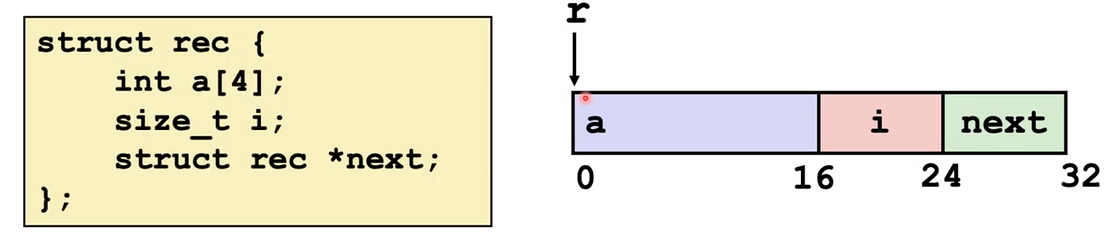
\includegraphics[scale = 0.45]{./figures/struct}
\end{figure}

An example of a struct is a Linked List:
\begin{figure}[h]
        \centering
        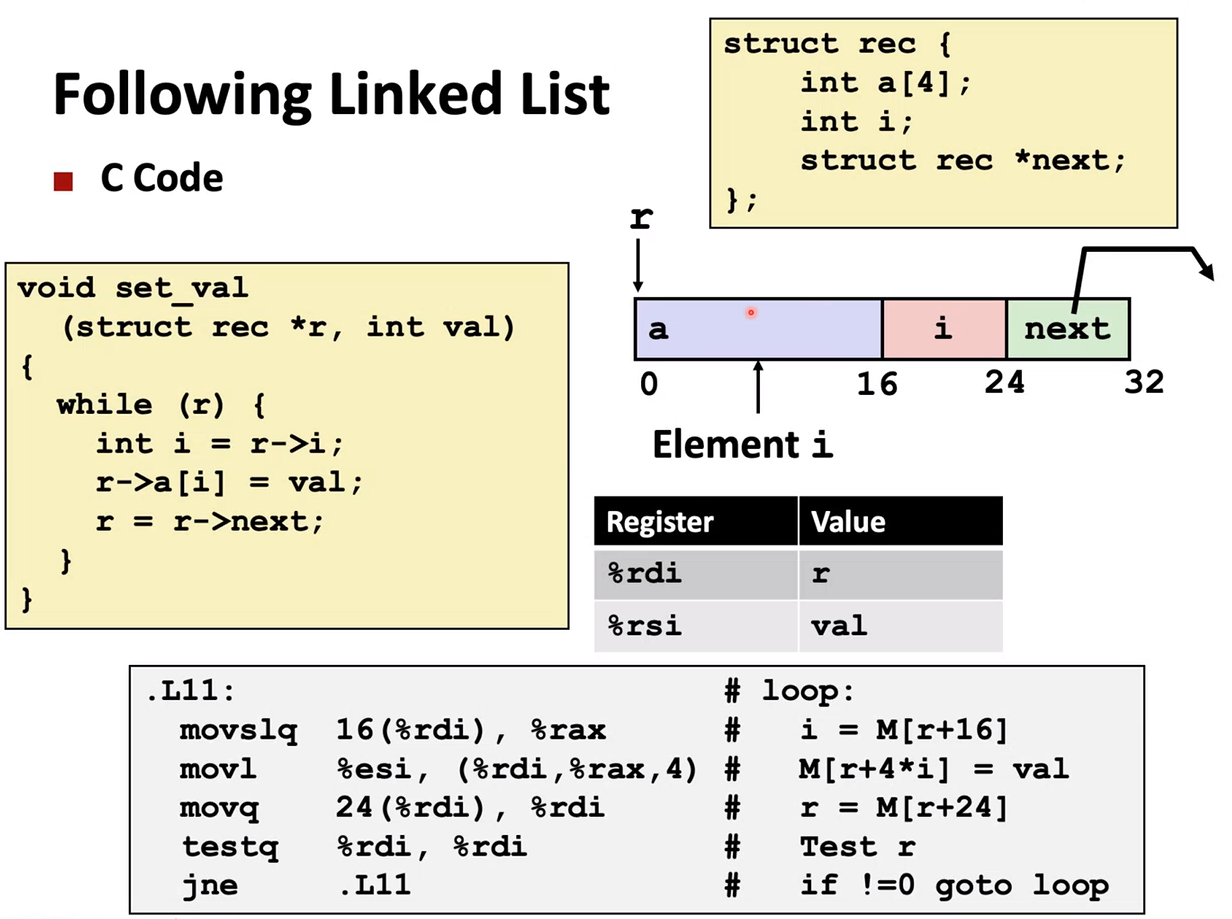
\includegraphics[scale = 0.4]{./figures/linkedlist}
\end{figure}

\subsection*{Structures \& Alignment}
An unaligned structure is a structure like in the previous example, where the 
amount of allocated space is not uniform. A struct with Aligned data is one where each
field is a multiple of a given number. (typically 2, 4, or 8)
\begin{figure}[h]
        \centering
        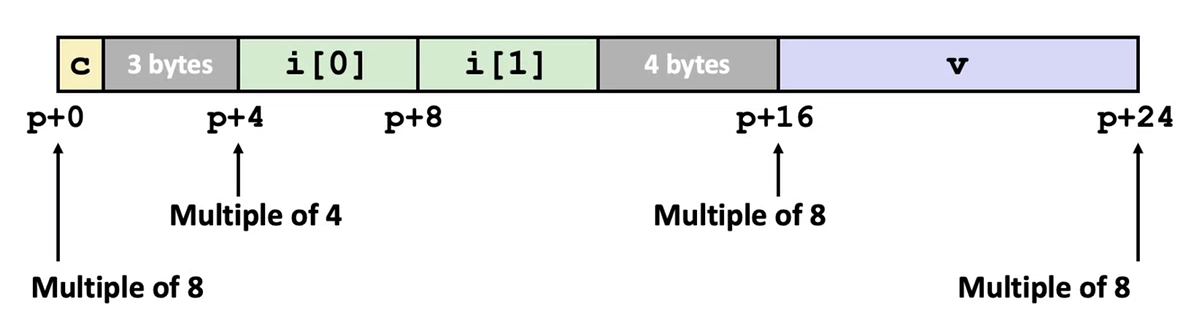
\includegraphics[scale = 0.4]{./figures/aligned}
\end{figure}

The reason this is done is that, without alignment, it is very difficult to read and write to
a struct. Note, the grey blocks are added by the compiler to `pad' the smaller $int$ datatypes.
Alignment is required on some machines but is only advised for x86-64.
The alignment rules for the primitive types of C are:
\begin{figure}[h]
        \centering
        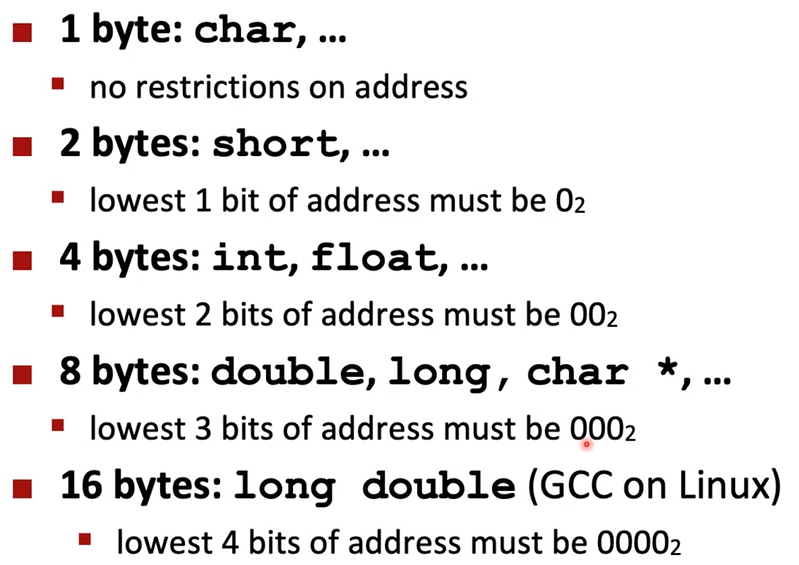
\includegraphics[scale = 0.5]{./figures/alignTable}
\end{figure}

Note: the number $K$ that is chosen to be the multiple for the rest of the fields is the 
number of bytes in the largest field. (see the above example with  \texttt{v})

Changing the order of the fields in the structure declaration changes their position in
memory. The convention is to declare the largest field first and progress to the smallest.
This can be seen in the reordering of the previous example:
\begin{figure}[h]
        \centering
        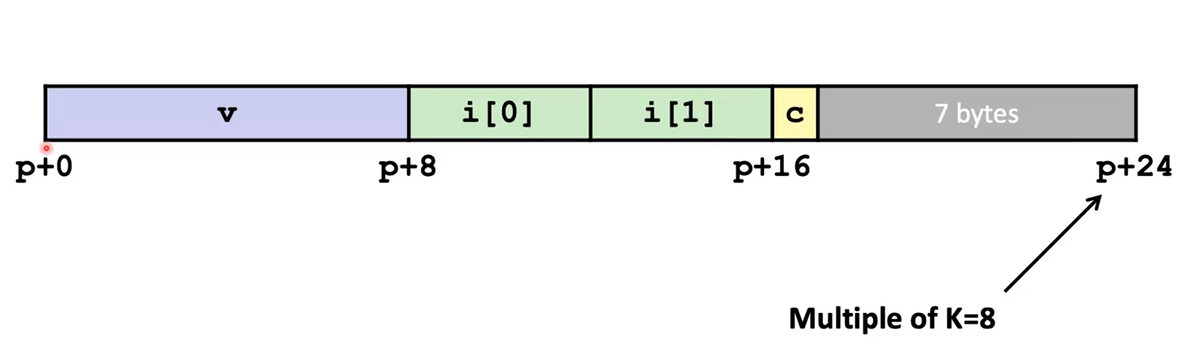
\includegraphics[scale = 0.4]{./figures/alignArrange}
\end{figure}

This convention can (but not always) result in less space in memory being used by the
structure.
\begin{figure}[h]
        \centering
        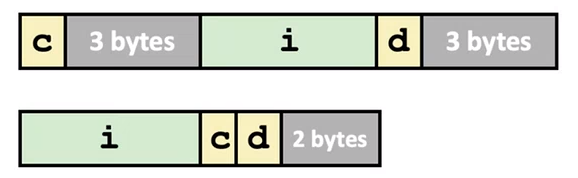
\includegraphics[scale = 0.4]{./figures/alignEx}
\end{figure}

\section*{Unions}
A structure is always contiguous, whereas a \textbf{Union} is not.
Space is allocated according to the largest element in the Union like so:
\begin{figure}[h]
        \centering
        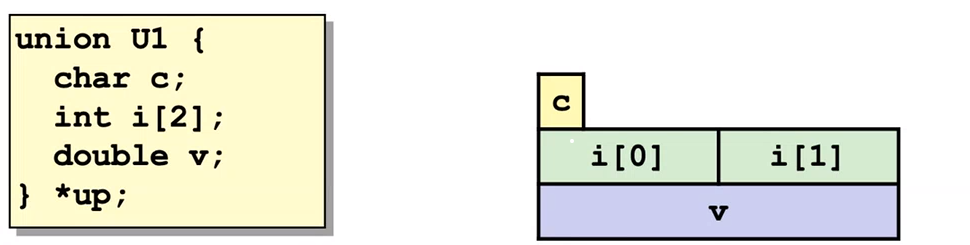
\includegraphics[scale = 0.4]{./figures/union}
\end{figure}
\pagebreak

As an example, below is a program that uses a union to access the bit pattern of a float:
\begin{figure}[h]
        \centering
        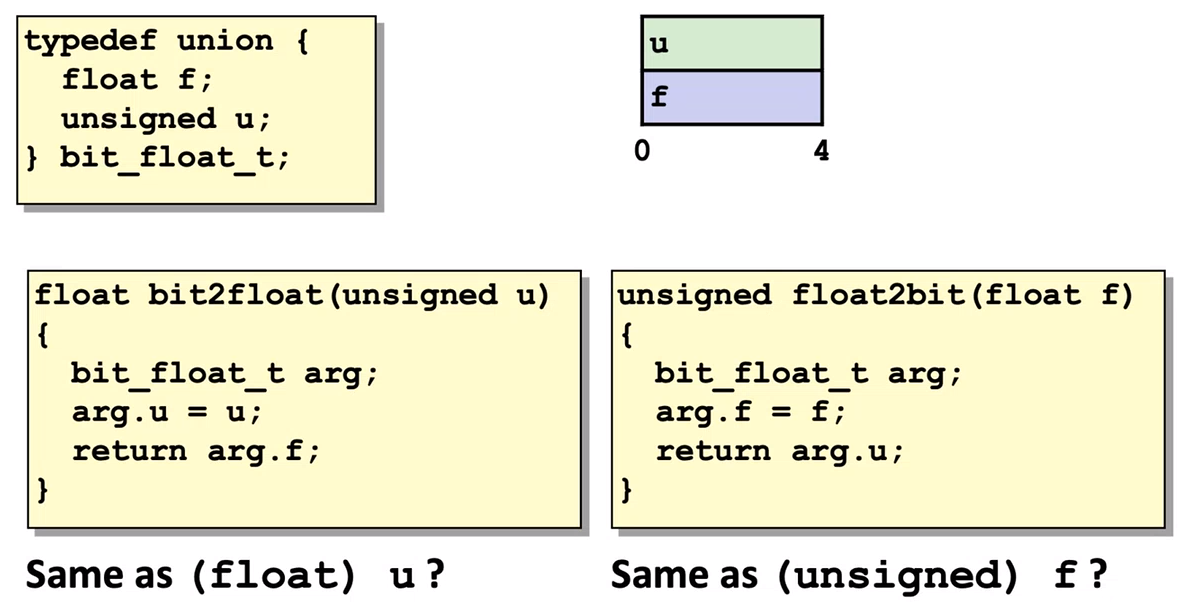
\includegraphics[scale = 0.4]{./figures/unionEx}
\end{figure}

In essence, a union stores 1 sequence of bits and calling its fields define how the stored 
sequence should be interpereted. 

The common usage of this datatype is to translate between machines / architectures.
It is also very useful for switching between signed and unsigned ints.

\section*{Floating Point}
Historically, there have been many ways of storing Floats.
\begin{itemize}
        \item x87 FP - very ugly \& old
        \item SSE FP - supported by x86 since 2000. Particularly good with vectors
        \item AVX FP - hot off the presses! Similar to SSE
\end{itemize}

Within SSE there are 16 registers (\texttt{\%xmm0,\ldots,\%xmm15}) to store information. Each register can hold anywhere from 
up to 16 single byte ints to up to 2 double precision floats.
\pagebreak

Operations are applied to floats like so:
\begin{figure}[h]
        \centering
        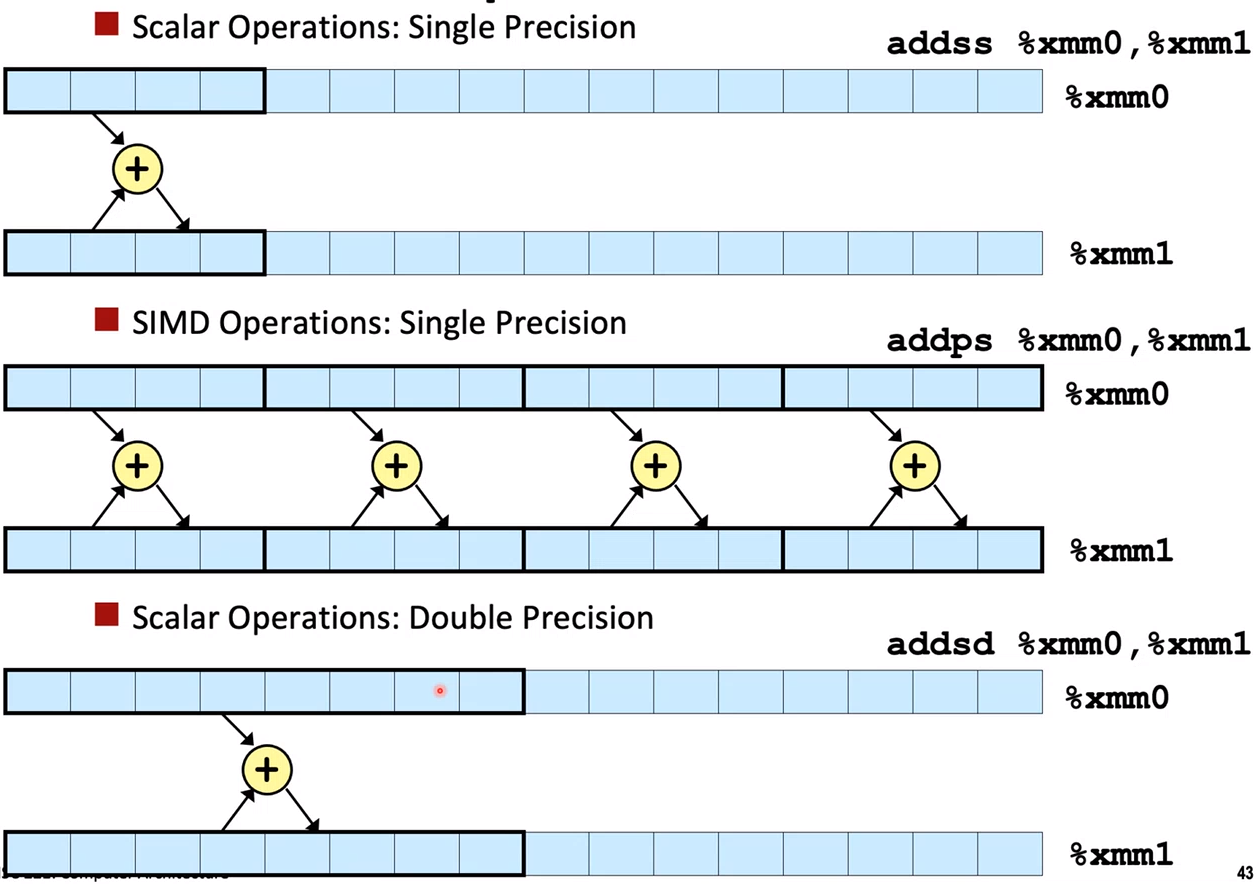
\includegraphics[scale = 0.4]{./figures/floatOps}
\end{figure}

\subsection*{Float Basics}
Within floating point operations, arguments are passed as \texttt{\%xmm0,\ldots,\%xmmN}.
The results are returned in \texttt{\%xmm0}.
Note that all \texttt{XMM} registers are caller saved.
\begin{figure}[h]
        \centering
        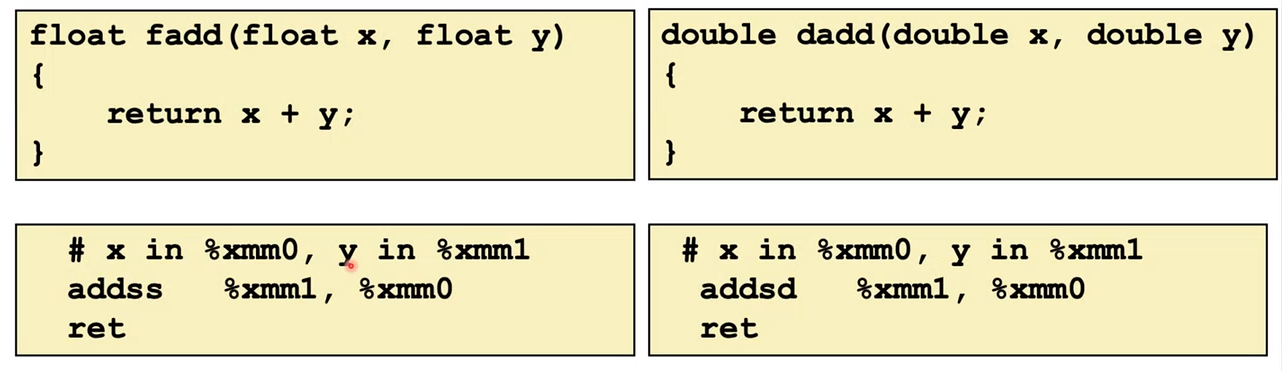
\includegraphics[scale = 0.3]{./figures/floatBasics}
\end{figure}

\subsection*{Float Memory Referencing}
in FP arithmetic, int and float arguments are passed in regular registers. FP values are 
passed in XMM registers. To move data between the two, there are specific \texttt{mov} 
instructions for doing so.
\begin{figure}[h]
        \centering
        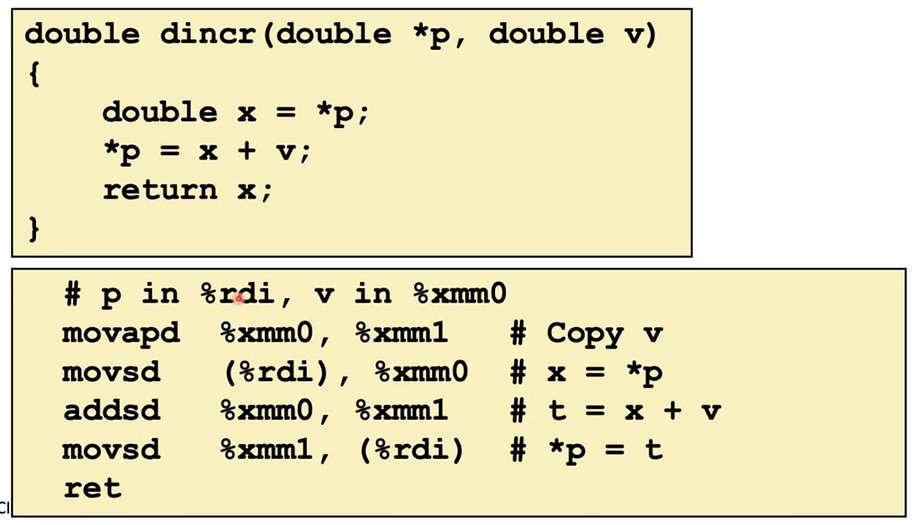
\includegraphics[scale = 0.4]{./figures/floatMov}
\end{figure}

\paragraph{more info about Floating Points}
There are alot of different operations and formats of operations for FP's so it can get 
complicated. Comparisons between FP's are done with \texttt{ucomiss, ucomisd} but the 
flags used ($CF, ZF, PF$) are the same as previously covered. There are also ways
of making an XMM register be constant.

\end{document}

